\section{Mechanical proofs of properties of Sturmian words}\label{sec:specific-theorems}

In this section we expand on the study done in \reed{Fibonacci word paper} with several new values for $\alpha$: $\sqrt{2}$ and $\sqrt{3}$.
We use these theorems to show the capabilities of our approach and to provide inspiration into what sorts of generalizations we may investigate using our new automata for $k$-bounded Sturmian words.

The words $\Ctwo$ and $\Cthree$ start as shown below:

\begin{itemize}
    \item[$\Ctwo$:] $01010010100101 \ldots$
    \item[$\Cthree$:] $11011101110110 \ldots$
\end{itemize}

%%%%%%% Section 3.1 %%%%%%%
\subsection{Aperiodicity}
%%%%%%% Theorem 4 %%%%%%%

We start with the well-known theorem that Sturmian words are not ultimately periodic \reed{cite}.
We check for $\Ctwo$ and $\Cthree$.

\begin{theorem}\label{thm:ulti_period_C}
The \word{}s $\Ctwo$ and $\Cthree$ are not ultimately periodic.
\end{theorem}
\begin{proof}
We construct the predicate that is true when infinite \word $C$ is ultimately periodic with period $p$:

\[(p\ge 1) \wedge \exists n~ \forall i \ge n ~ C[i] = C[i+p]\]

Using Walnut on $\Ctwo$ and $\Cthree$, we get an automaton that accepts the empty language. It follows that $\Ctwo$ and $\Cthree$ are not ultimately periodic.
\end{proof}

\subsection{Palindromes and antipalindromes}
\eric{Use this definition style?}
\begin{definition}
A string $s$ is a \emph{palindrome} if its reverse is the same as itself, that is, when $s = s^R$.
\end{definition}
\begin{definition}
A string $s$ is \emph{mirror invariant} if for any factor $x$, the reverse $x^R$ is also a factor of $s$.
\end{definition}
\begin{definition}
A string $s$ is an \emph{antipalindrome} if its reverse is the complement of itself, that is, when $s = \overline{s^R}$.
\end{definition}
\begin{theorem}
$\Ctwo$~ and $\Cthree$ contains antipalindromes of all lengths.
\end{theorem}
For any given string $C$, the following predicate specifies if the substring $C[i..i+n-1]$ is a palindrome:
\[\forall t<n ~C[i+t] = C[i+n-1-t]\]
Using Walnut, we checked that there are palindromes of all lengths in $\Ctwo$~ and $\Cthree$.
%%%%%%%%%%%%%%%%%%%%%% Theorem 13 %%%%%%%%%%%%%%%%%%%%%%
\begin{theorem}
$\Cthree$ ~contains exactly one palindrome of length $n$ if and only if $n$ is odd. 
\end{theorem}
\begin{proof}
The following predicates is true when there is exactly one palindrome of length $n$ in string $C$. 
\begin{multline*}
    \exists i \wedge (\forall t<n \implies C[i+t] = C[i+n-1-t] \wedge \\
    \forall j (\forall t<n \implies C[j+t] = C[j+n-1-t] \implies \forall u<n \implies C[i+u] = C[j+u]))
\end{multline*}
We ran the formula for $\Ctwo$ ~and $\Cthree$. The resulting automaton is shown in the following figures

\begin{figure}[h!]
\vspace{10mm}
	\begin{minipage}{0.45\textwidth}
      \centering
      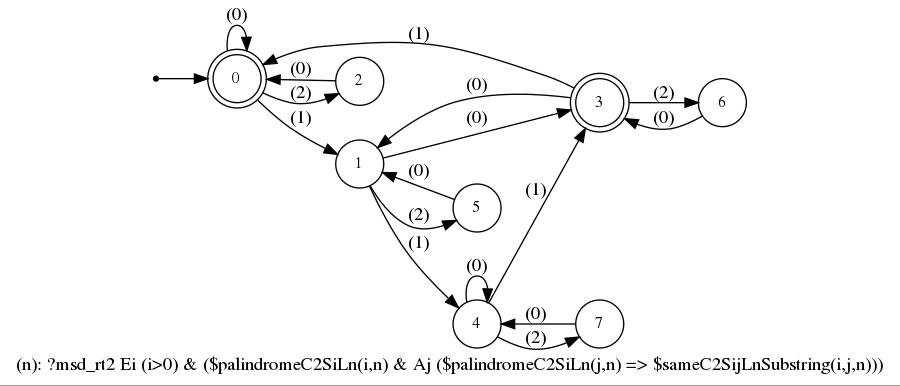
\includegraphics[width=\linewidth]{sturmian_word_paper/paper_images/theorem13_C2.jpg}
      \caption{Length with exactly one palindrome in $\Ctwo$}
      \centering

  	\end{minipage}%
    \hspace{0.05\textwidth}
    \begin{minipage}{0.45\textwidth}
      \centering
      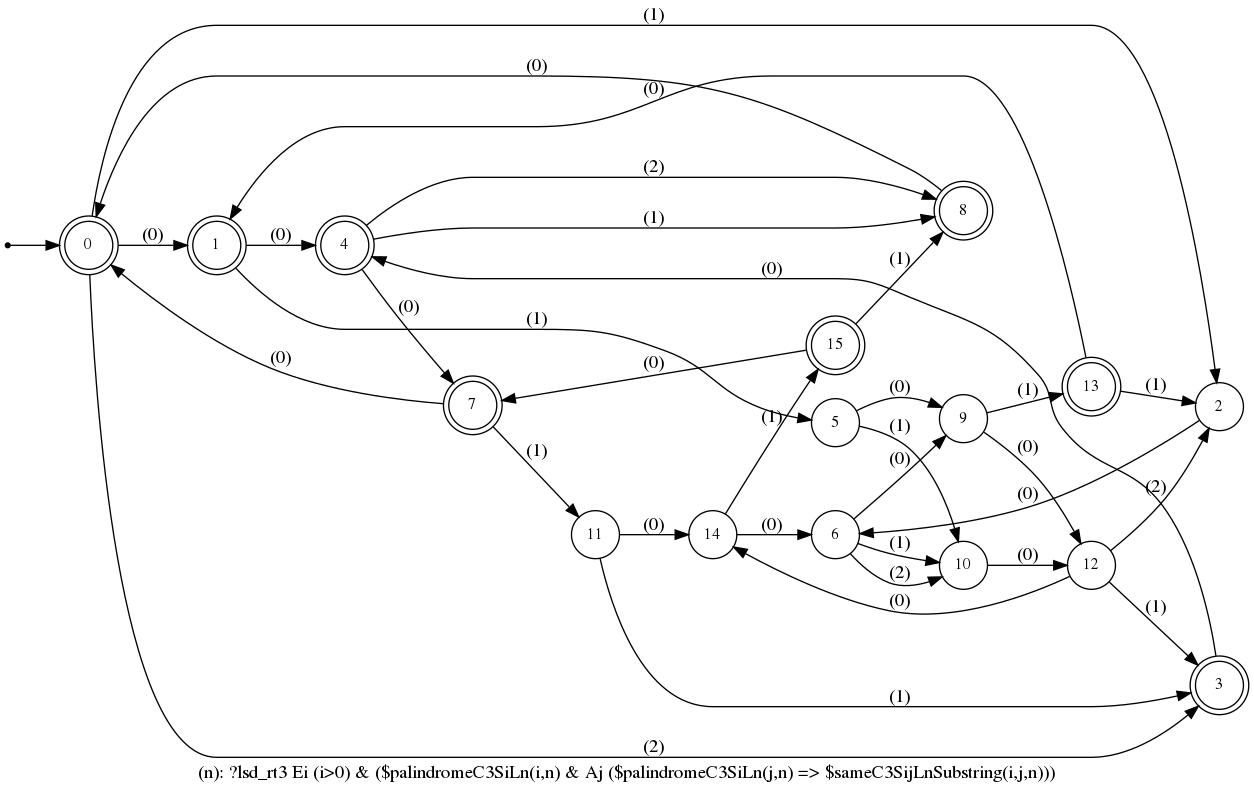
\includegraphics[width=\linewidth]{sturmian_word_paper/paper_images/theorem13_C3.jpg}
      \caption{Length with exactly one palindrome in $\Cthree$}
      \centering

    \end{minipage}
\end{figure}

\eric{Crop images so that they look better.}

The predicate that accepts even numbers $n$ is $\exists i ~n=2i$. We ran this predicate in Walnut and found that the automaton are the same. 
\end{proof}
\eric{Not important now: Check for k-bounded, does it depend on the slope?}
%%%%%%%%%%%%%%%%%%%%%% Theorem 15 %%%%%%%%%%%%%%%%%%%%%%

\begin{theorem}
$\Ctwo$ and $\Cthree$ are mirror invariant. 
\end{theorem}
\begin{proof}
The following predicate accepts $n$ if all substring $s$ of $C$ of length $n$ that is also in $C$. \[\forall i \exists j \forall t<n C[i+t] = C[j+n-1-t]\]
The resulting automaton accepts all integer $n$, suggesting that $\Ctwo$~ and $\Cthree$ ~are both mirror invariant. 
\end{proof}

\begin{theorem}
The only nonempty antipalindromes in $\Ctwo$ are 01, 1001, and 010010.\\
The only nonempty antipalindromes in $\Cthree$ are 01 and 10.
\end{theorem}
\begin{proof}
The following predicate is true when there is an antipalindrome of length  $n$.
\[\forall t<n~ C[i+t] \ne C[i+n-1-t]\]

Here is the result automaton given by Walnut when $C=\Ctwo$ and $C = \Cthree$.

\begin{figure}[h!]
\vspace{10mm}
	\begin{minipage}{0.45\textwidth}
      \centering
      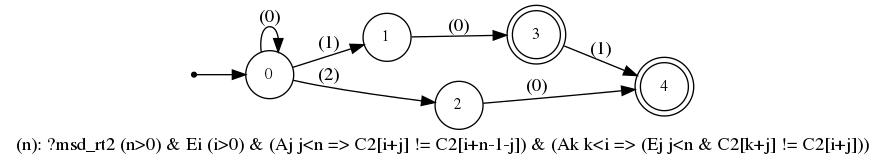
\includegraphics[width=\linewidth]{sturmian_word_paper/paper_images/theorem16_nC2.jpg}
      \caption{Length of antipalindromes in $\Ctwo$}
      \centering

  	\end{minipage}%
    \hspace{0.05\textwidth}
    \begin{minipage}{0.45\textwidth}
      \centering
      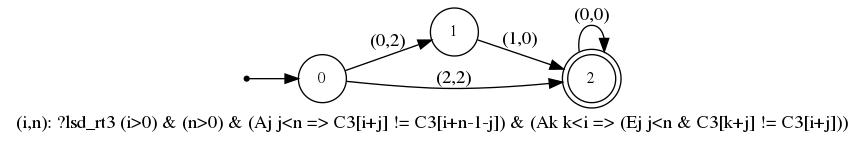
\includegraphics[width=\linewidth]{sturmian_word_paper/paper_images/theorem16.jpg}
      \caption{Length of antipalindromes in $\Cthree$}
      \centering

    \end{minipage}
\end{figure}

The above automata implies that there are only antipalindromes of length 2, 4, and 6 in $\Ctwo$, and antipalindromes of length 2 in $\Cthree$. Therefore, together with the fact that there are no substrings 000 and 11 in $\Ctwo$ \eric{cite this}, the antipalindromes in $\Ctwo$ can only be 01, 1001, and 010010, and the antipalindromes in $\Cthree$ can only be 01 or 10. An example of each can be found within the first 10 digits of $\Ctwo$ and $\Cthree$, presented at the beginning of this section.
% An example of substring 01 can be found at $\Cthree [3,4]$, and an example of substring 10 can be found at $\Cthree [2,3]$.
\end{proof}

\subsection{Special factors}
Next we will prove that \Ctwo and \Cthree \ have exactly n + 1 distinct factors of length n, for each n $\geq$ 0.  This implies that there is exactly one factor x of each length n with the property that both x0 and x1 are factors. Such a factor is called right-special or just special.  We can write a predicate that expresses the assertion that the factors \Ctwo[i..i+n-1] and \Cthree[i\ldots i+n-1] are the unique special factors of length n, and furthermore, that they are the first occurrences of those factors where C = \Ctwo \ or \Cthree, as follows: \\
\begin{equation*}
    (\forall i'< i\ \exists s < n\ C[i'+s] \ne C[i+s])\ \wedge\ \exists j\ \exists k\ ((\forall t < n\ C[j+t] = C[i+t])\ \wedge\ (\forall u < n\ C[k+u]=C[i+u])  
\end{equation*} 
$\wedge\ (C[j+n] \ne C[k+n]))$ \\

\begin{theorem}
The automaton depicted in the figure below accepts the language {$(i,n)_{\Ctwo}$: the factor \Ctwo[i\ldots i+n-1] is the first occurrence of the unique special factor of length n}.
\end{theorem}

\begin{figure}[h]
    \centering
    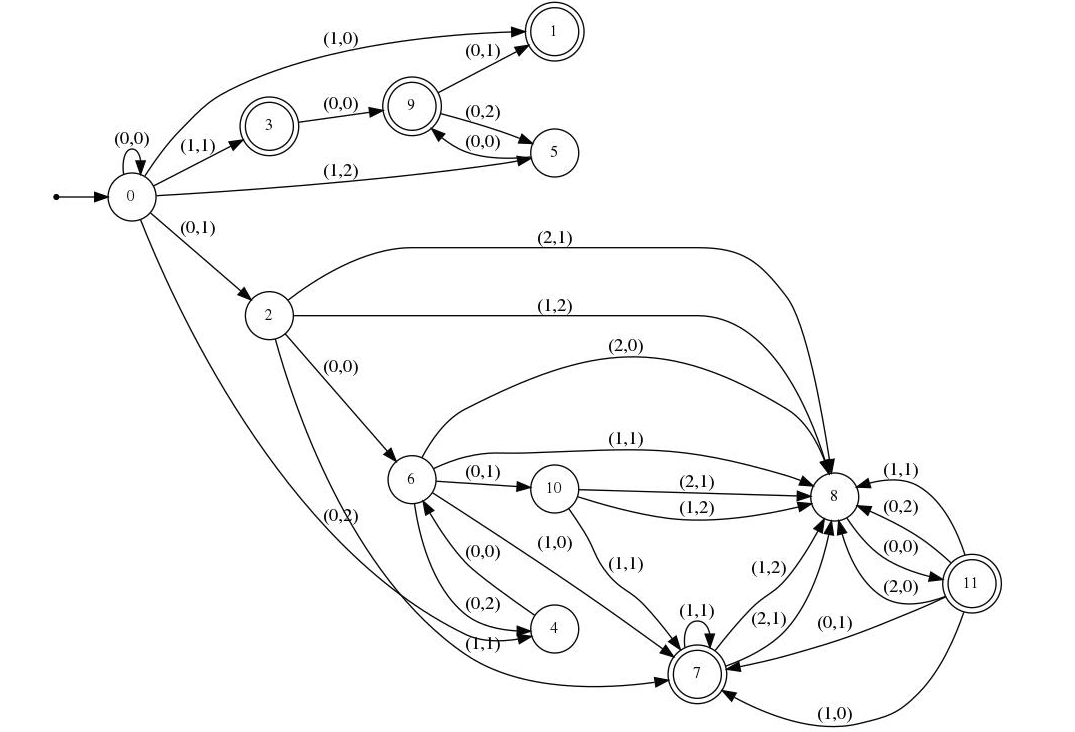
\includegraphics[width=\textwidth]{sturmian_word_paper/paper_images/rt2theorem17.png}
    \caption{Automaton accepting first positions and lengths of special factors in $\Ctwo$}
\end{figure} 
Furthermore, we know that,
\begin{theorem}
The unique special factor of length n is $C[0\ldots n-1]^{R}$, where C = \Ctwo\ or \Cthree
\end{theorem}
\begin{proof}
We create a predicate which says that if a factor is special then it matches $C[0\ldots n-1]^{R}$. When we run this we discover that all lengths are accepted for C = \Ctwo\ and \Cthree.
\end{proof}
\subsection{Least periods}
Let $P$ denote the assertion that
\textit{n} is a period of the factor 
$C$\big[\textit{i \ldots j}\big], where $C= \Ctwo \text{ or } \Cthree$, as follows:

\begin{equation*}
    P(n,i,j) = C\big[\textit{i \ldots j} \big] = C\big[\textit{i}+\textit{n..j}\big]
    = \forall t,\ \text{with}\  i\leq t \leq j-n\  \text{we have}\  C\big[\textit{t}\big] = C\big[\textit{t}+\textit{n}\big].
\end{equation*}
\\
Using $P$, we can express the predicate $LP$ where $n$ is the least period of $C$\big[\textit{i..j}\big]:

$$LP(n,i,j) = P(n,i,j) \text{ and } \forall n' \text{ with } 1 \leq n' < n \  \neg P(n',i,j)$$

Lastly, we can express the predicate that n is the least period as follows:

$$L(n) = \exists i,j \geq 0 \text{ with } 0 \leq i+n \leq j-1 \  LP(n,i,j)$$


Using an implementation of the last expressions, we can prove the following theorem:

\begin{theorem}
If a word $w$ is a nonempty factor of the $C$ word, then the least period of $w$ is a Pell number $C_{n}$ for $n \geq 2$. The following periods occurs.
\end{theorem}

\begin{proof}
After running the above functions, the resulting automaton accepts $10^{+}+110^{*}$, which corresponds to the Pell numbers as factors of $C_{\sqrt{2}}$ for $n\geq2$. For $C_{\sqrt{3}}$ the following automaton is given. The following Automata corresponds to $C_{\sqrt{2}}$ and $C_{\sqrt{3}}$ respectively:  \reed{Not just the pell numbers}

\begin{figure}[h!]
\vspace{10mm}
	\begin{minipage}{0.45\textwidth}
      \centering
      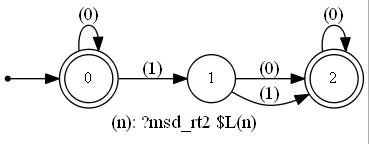
\includegraphics[width=\linewidth]{sturmian_word_paper/paper_images/rt2Theorem19.jpg}
      \caption{Theorem 4.11 $\Ctwo$}
      \centering

  	\end{minipage}%
    \hspace{0.05\textwidth}
    \begin{minipage}{0.45\textwidth}
      \centering
      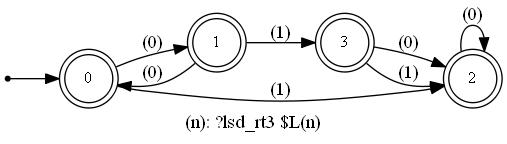
\includegraphics[width=\linewidth]{sturmian_word_paper/paper_images/rt3Theorem19.jpg}
      \caption{Theorem 4.11 $\Cthree$}
      \centering

    \end{minipage}
\end{figure}
\end{proof} 

\begin{theorem}\label{thm:lp-C2}
Let $n\geq1$ and define $l(n)$ to be the smallest integer that is the least period of the some length-n factor of $C_{\sqrt{2}}$. 
\end{theorem}\dago{Need to translate theorem for C2 and C3. This is theorem 20 from the Fibbonacci Paper}
\begin{proof}
An automaton was created accepting $(n,p)_{C_{\sqrt{2}}}$ and $(n,p)_{C_{\sqrt{3}}}$ respectively such that (a) there exists at least one length-$n$ factor of period \textit{p} and (b) for all length-$n$ factors $x$, if $q$ is a period of $x$, then $q\geq p$.

\begin{figure}[h!]
\vspace{10mm}
	\begin{minipage}{0.45\textwidth}
      \centering
      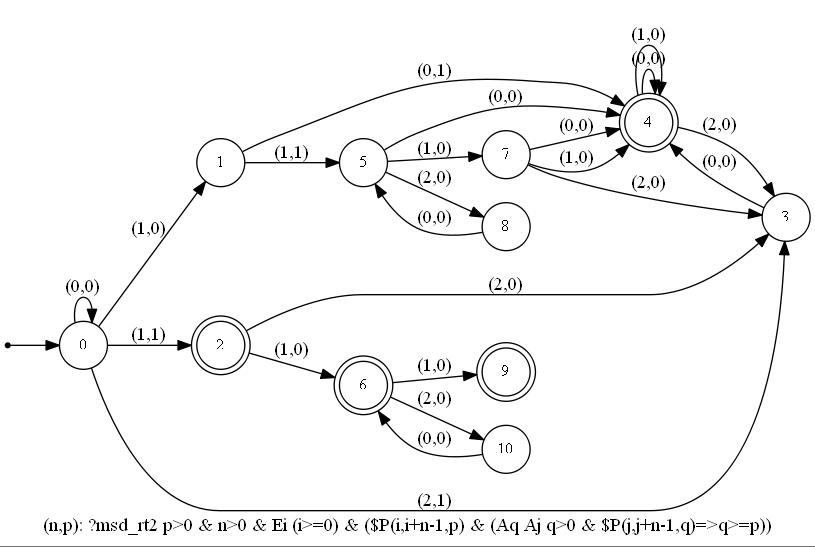
\includegraphics[width=\linewidth]{sturmian_word_paper/paper_images/rt2Theorem20.jpg}
      \caption{Theorem 4.12 $\Ctwo$}
      \centering

  	\end{minipage}%
    \hspace{0.05\textwidth}
    \begin{minipage}{0.45\textwidth}
      \centering
      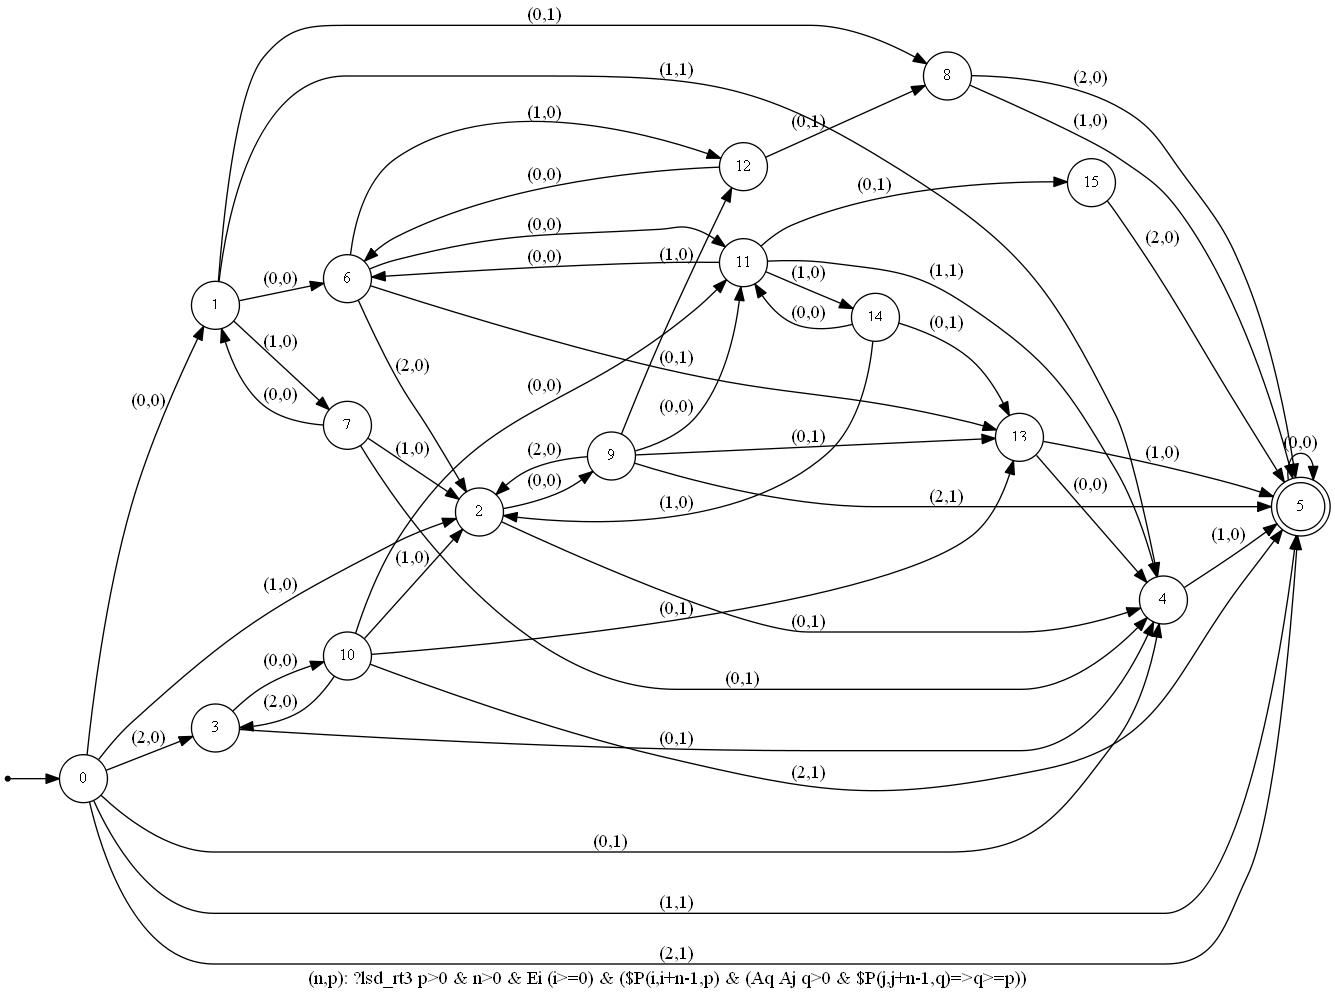
\includegraphics[width=\linewidth]{sturmian_word_paper/paper_images/rt3Theorem20.jpg}
      \caption{Theorem 4.12 $\Cthree$}
      \centering

    \end{minipage}
\end{figure}
\end{proof}

\subsection{Quasiperiods}

An infinite word \textbf{a} is said to be \term{quasiperiodic} if there is some finite nonempty word $x$ such that $a$ can be completely ``covered" with translates of $x$. 
We study the stronger version of quasiperiodicity where the first copy of $x$ used must be aligned with the left edge of \textbf{w} and is not allowed to ``hang over"; these are called \term{aligned covers}. 
For us $\mathbf{a} = a_{0}a_{1}a_{2}...$ is quasiperiodic if there exists $x$ such that for all $i>0$ and $i>n$ there exists $j>0$ with $i-n<j\leq i$ such that $a_{j}a_{j+1}...a_{j+n-1}=x$, where $n=|x|$. Such an $x$ is called a \term{quasiperiod}. 
Note that the condition $j>0$ implies that, in this interpretation, any quasiperiod must actually be a be a prefix of \textbf{a}.

\begin{theorem}
A nonempty length-$n$ prefix of $\Ctwo$ is a quasiperiod of $\Ctwo$ if and only if $n$ is not in the form $P_n - 1$ or $P_n + P_{n-1} - 1$, where $P_n$ are Pell numbers.
\end{theorem}

\begin{proof}
We write a predicate for the assertion that the length-$n$ prefix is a quasiperiod: 
\begin{equation*}\label{eqn:quasiperiod-def}
    \forall i>0 ~ \exists j > 0 ~ \text{with} ~ \text{and} ~ i-n<j\leq i ~ \text{such that} ~ \forall t>0 ~ \text{and} ~ t \leq n ~ C_{\sqrt{2}}[t] = C_{\sqrt{2}}[j+t]
\end{equation*}

After running the predicate in Walnut, we get the following automaton asserting the previous theorem:

\end{proof}
%\dago{Tried adding the pictures rt2Theorem21 and rt3Theorem21 to the proof environment, but they ended up somewhere else in the paper. I tried following the example as in section 4.4 and 4.7 where the pictures are added side by side}

\subsection{Recurrence, uniform recurrence, and linear recurrence}
\eric{Add reference}
A \factor $x$ of infinite \word $C$ is said to be \term{recurrent} if it occurs infinitely many times in $C$. 
An infinite \word $C$ is \term{recurrent} if every factor of $C$ is recurrent. 
A \factor $x$ is \term{uniformly recurrent} if there exists a length $n = n(x)$ such that every factor of length $n$ contains $x$.
An infinite word is uniformly recurrent if all factors of its factors are uniformly recurrent.
If $n(x)$ is in $O(x)$ for all factors $x$, then $C$ is linearly recurrent. 
\eric{Is that the correct language?}

Notice that linear recurrence implies uniform recurrence and recurrence.

\begin{theorem}
$\Ctwo$ and $\Cthree$ are linearly recurrent. 
\end{theorem}

\begin{proof}
The following predicate is true if and only if $n(x) \leq M|x|$ for all factors $x$.

\[\forall n,i,j ~\exists s ~(j\le s\le j+Mn) \wedge (\forall p<n (C[s+p] = C[i+p]))\]

To verify the theorem, we choose $C = \Ctwo$ or $\Cthree$ and choose $M=4$. In both cases, the resulting automaton is a true automaton.  
\end{proof}

\subsection{Lyndon words}

A nonempty word $x$ is a \textit{Lyndon word} if it is lexicographically less than all of its nonempty proper prefixes. For example, in $C_{\sqrt{2}}$, 120 is a Lyndon word as it is lexicographically less than its rotations, 201 and 012, in lsd.

\begin{theorem}
In $C_{\sqrt{2}}$ and $C_{\sqrt{3}}$, there exists a Lyndon factor of all lengths n.
\reed{Are we sure about this? Did we ensure that all the indices are bigger than 0?}
\end{theorem}

\begin{proof}
We consider the predicate specifying that there is a factor of length n that is Lyndon:

\begin{equation*}
    \exists i, 1 \leq i, \forall j, 1 \leq j < n, \exists t < n-j  (\forall u < t C_{\sqrt{2}}[i + u] = C_{\sqrt{2}}[i + j + u]) \wedge C_{\sqrt{2}}[i + t] < C_{\sqrt{2}}[i + j + t]
\end{equation*}

When we run this predicate, we produce the following automata for $C_{\sqrt{2}}$ and $C_{\sqrt{3}}$ respectively:

\begin{figure}[h!]
\vspace{10mm}
	\begin{minipage}{0.45\textwidth}
      \centering
      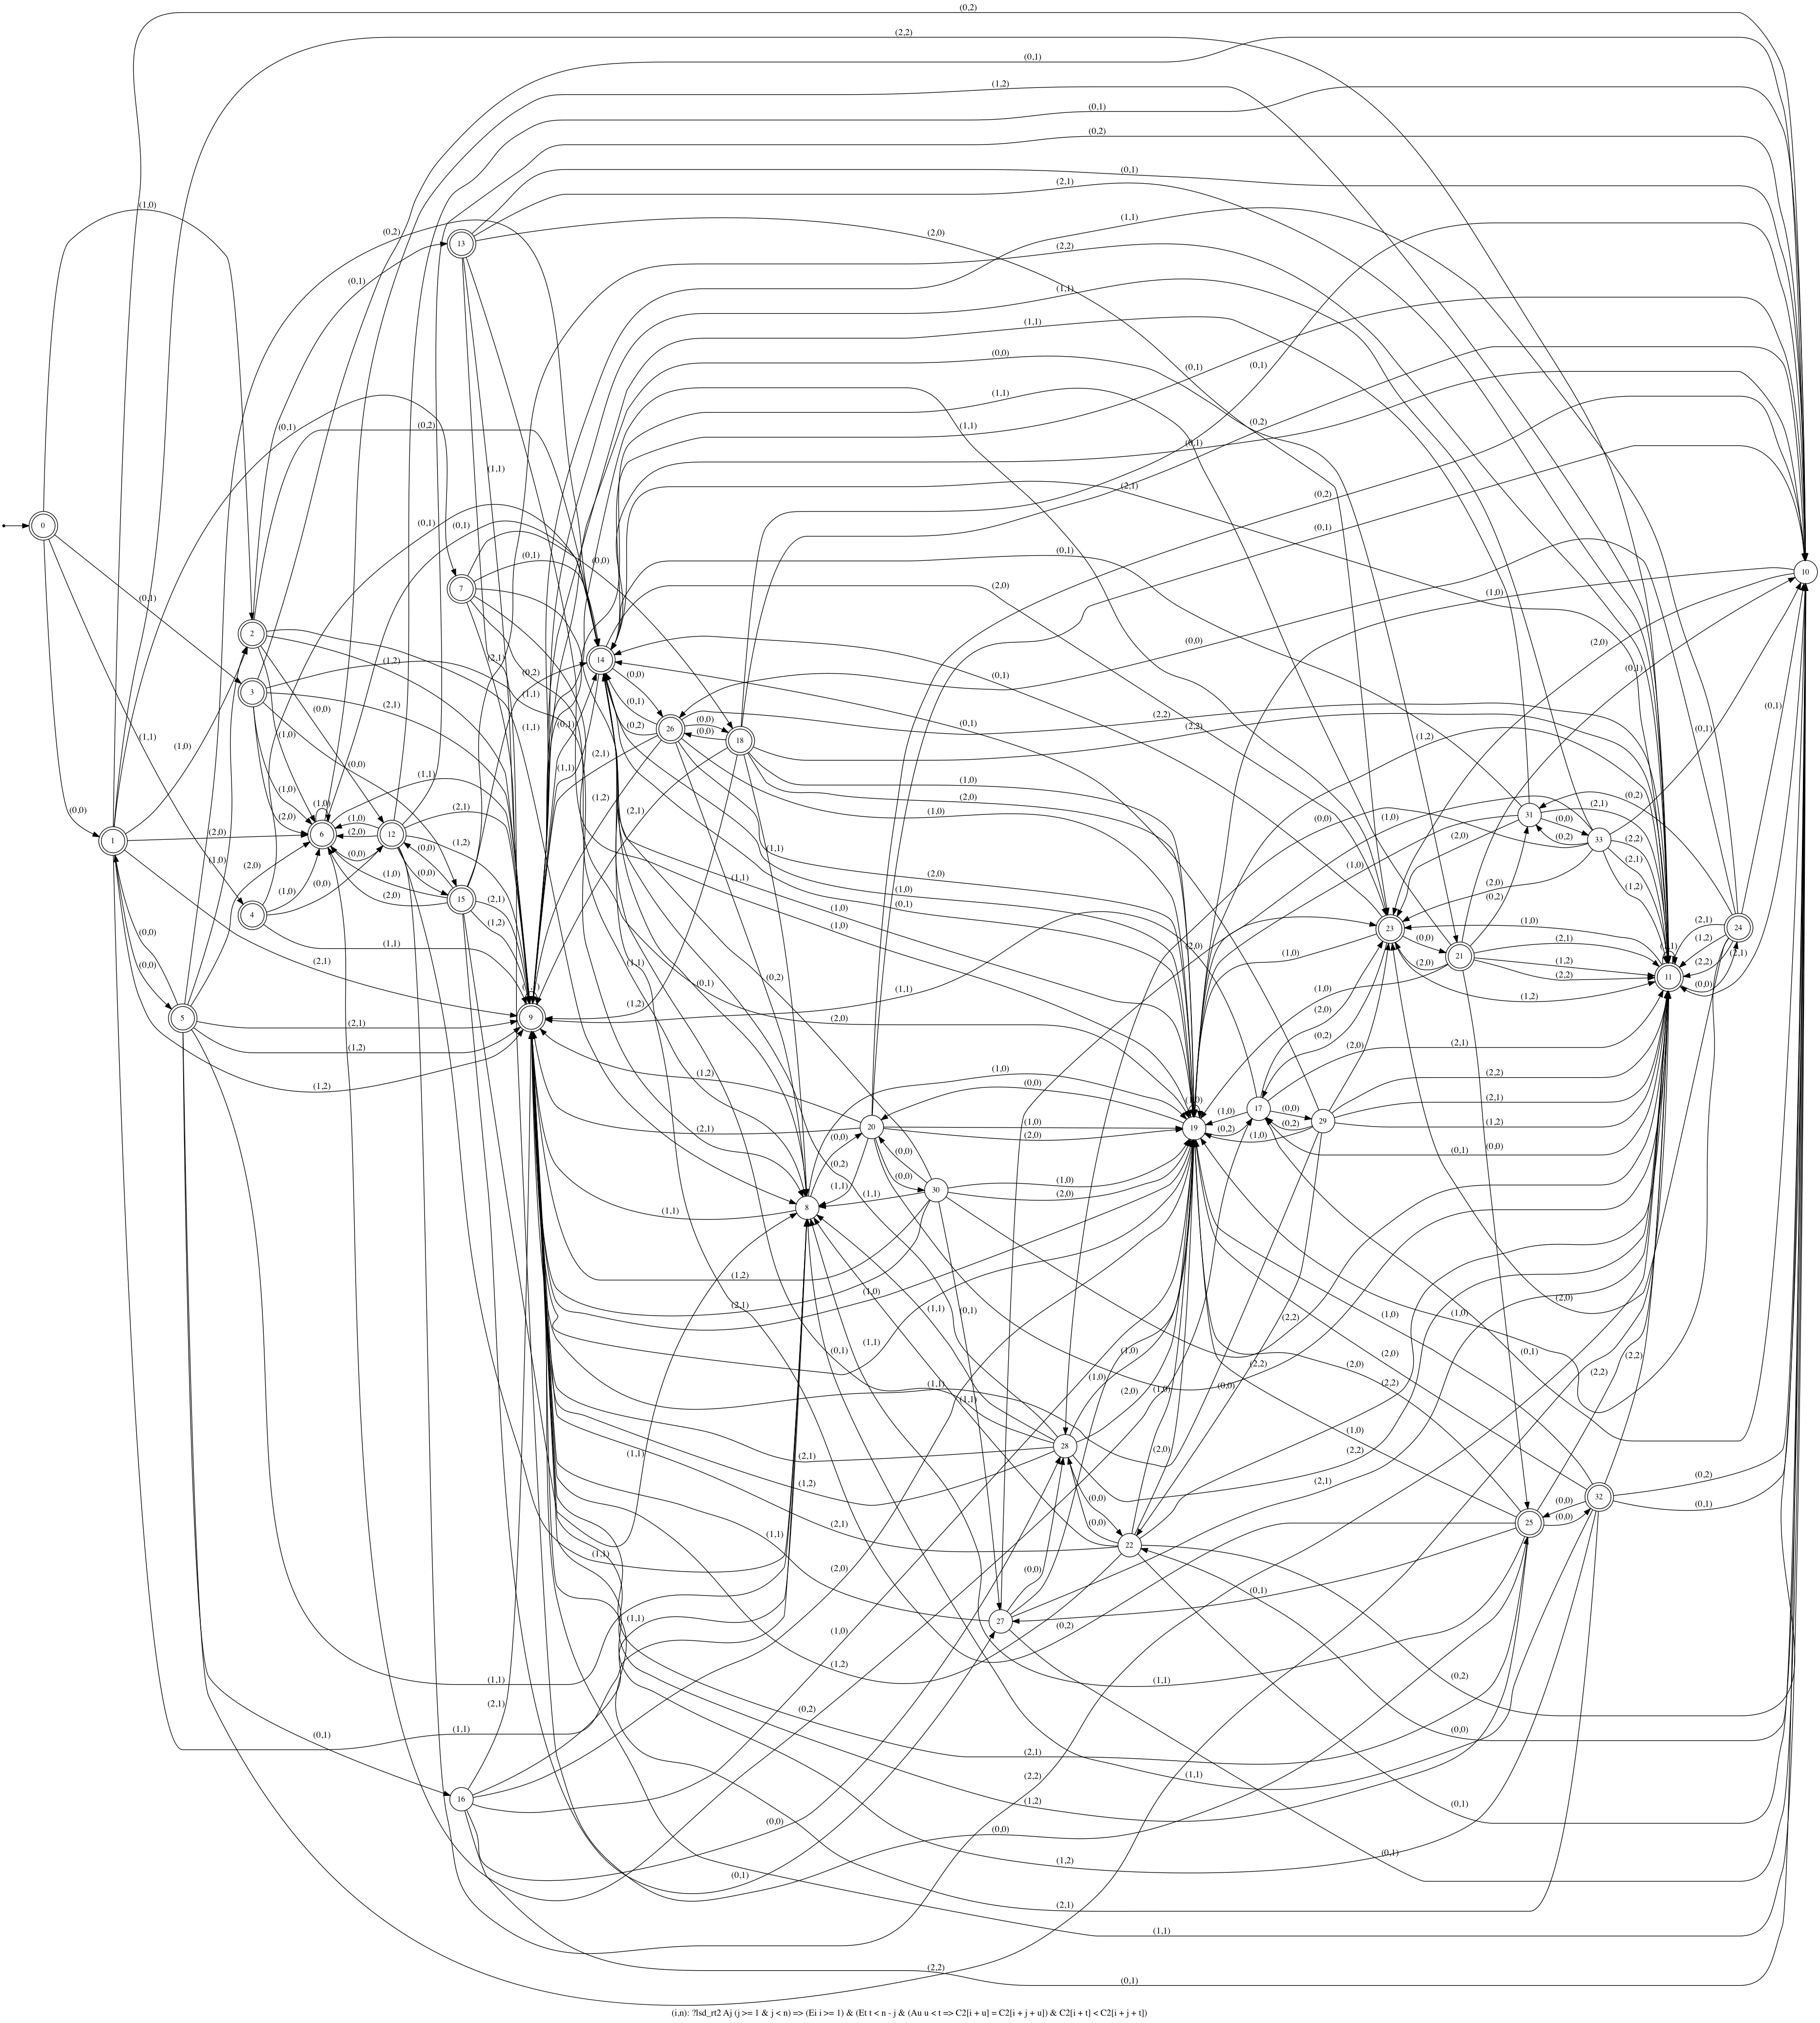
\includegraphics[width=\linewidth]{sturmian_word_paper/paper_images/root2theorem25.jpg}
      \caption{Automaton specifying that there is a factor of length n that is Lyndon in $\Ctwo$.}
      \centering

  	\end{minipage}%
    \hspace{0.05\textwidth}
    \begin{minipage}{0.45\textwidth}
      \centering
      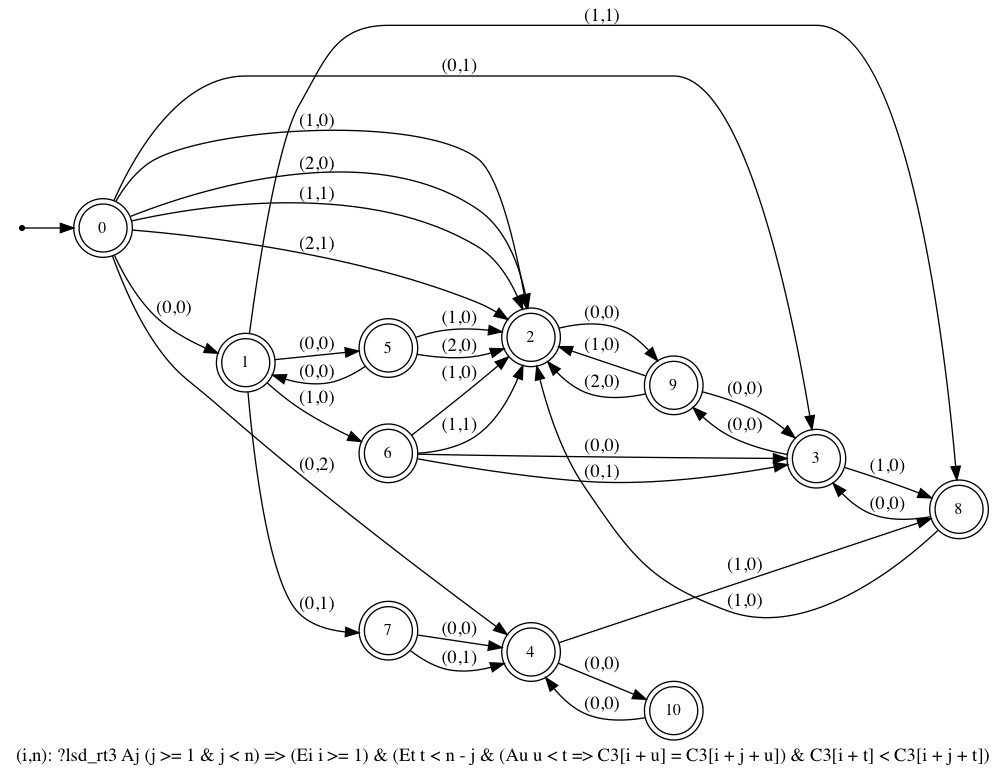
\includegraphics[width=\linewidth]{sturmian_word_paper/paper_images/root3theorem25.jpg}
      \caption{Automaton specifying that there is a factor of length n that is Lyndon in $\Cthree$.}
      \centering

    \end{minipage}
\end{figure}

We can then conclude that for all lengths $n$, there exists a Lyndon factor of length $n$ in $C_{\sqrt{2}}$ and $C_{\sqrt{3}}$.
\end{proof}

It can be seen that this result differs from the Fibonacci numeration system, where there exists a Lyndon factor of length $F_n$ for $n \geq 2$.

\begin{theorem}
For $n \geq 1$, every length-$n$ Lyndon factor of $C_{\sqrt{2}}$ or $C_{\sqrt{3}}$ is a conjugate of $C_{\sqrt{2}}(1, n)$ or $C_{\sqrt{3}}(1, n)$ respectively.
\end{theorem}

\begin{proof}
Using the previous predicate as a base, we can create the predicate specifying that every length-$n$ Lyndon factor is a conjugate of $\Ctwo(1, n)$. The resulting automata show that all lengths of n are accepted for $\Ctwo$ and $\Cthree$. A similar argument leads to the same result for $\Cthree$.
\end{proof}

\begin{figure}[h!]
\vspace{10mm}
	\begin{minipage}{0.45\textwidth}
      \centering
      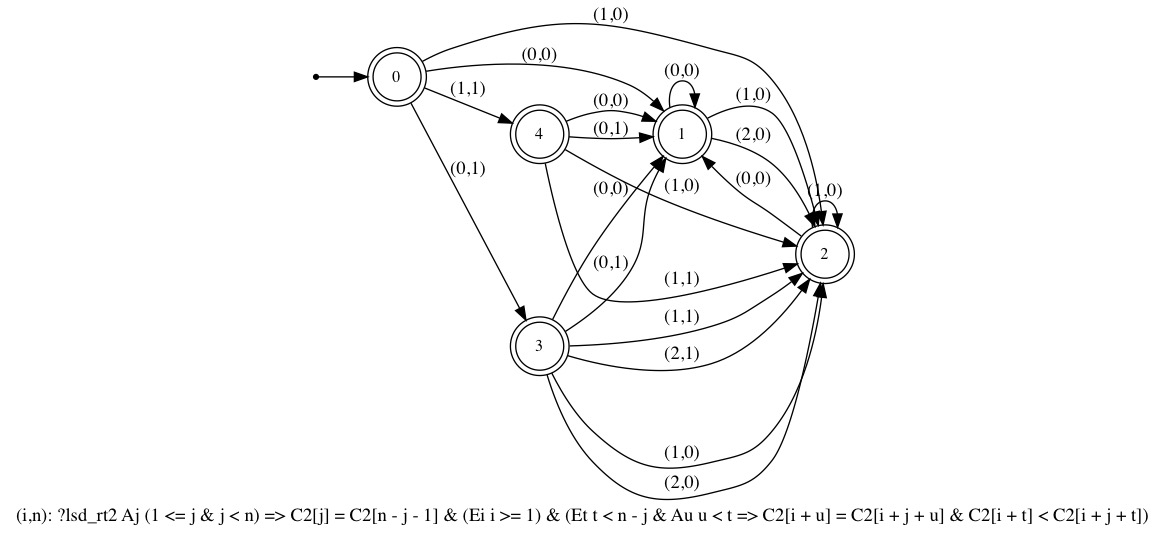
\includegraphics[width=\linewidth]{sturmian_word_paper/paper_images/root2theorem26.jpg}
      \caption{Automaton specifying that every Lyndon factor of length n is a conjugate of $\Ctwo(1, n)$.}
      \centering

  	\end{minipage}%
    \hspace{0.05\textwidth}
    \begin{minipage}{0.45\textwidth}
      \centering
      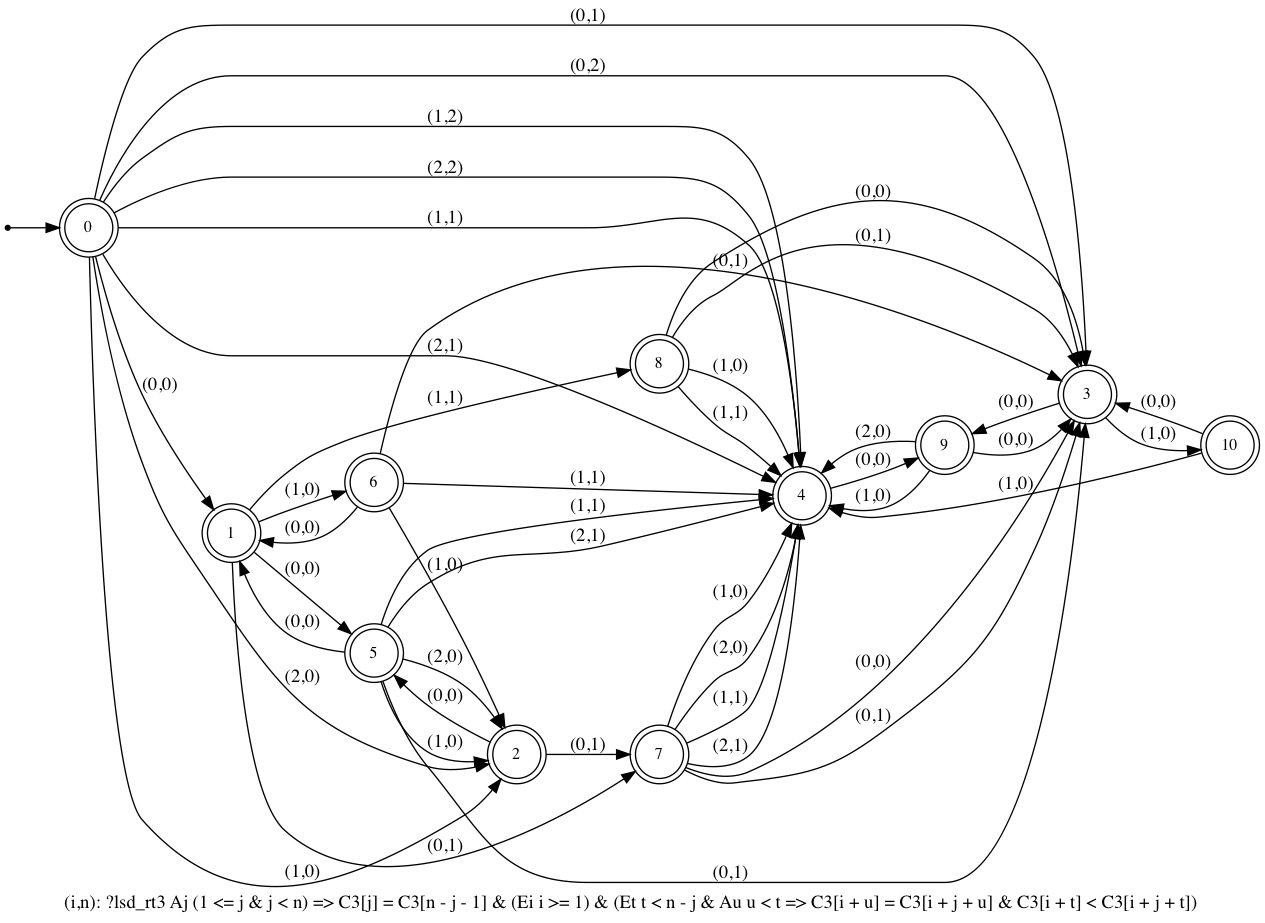
\includegraphics[width=\linewidth]{sturmian_word_paper/paper_images/root3theorem26.jpg}
      \caption{Automaton specifying that every Lyndon factor of length n is a conjugate of $\Cthree(1, n)$.}
      \centering

    \end{minipage}
\end{figure}

\subsection{Critical Exponents}
Define exp(\textit{w}) as $|\textit{w}|$/\textit{P}, where \textit{P} is the smallest period of \textit{w}. 
The \textit{critical exponent} of an infinite word \textbf{x}, is the supremum, over all factors $w$ of \textbf{x}, of exp(\textit{w}).

\begin{theorem}
The critical exponent of $C_{\sqrt{2}}$ is $4 + 2\sqrt{2}$.
\end{theorem}
\begin{proof}
\reed{Copy this up to the section about this}
As shown in Theorem~\ref{thm:lp-C2}, $\ell(n) = U_n(2,-1)$ for $V_n(2,-1) - 1 \leq n \leq V_{n+1}(2,-1) - 2$, where $U_n$ and $V_n$ are the Lucas sequences, defined in Section~\ref{sec:background}.
Therefore, the critical exponent of $C_{\sqrt{2}}$ is given by $\lim_{n \to \infty} \frac{V_{n+1}(2,-1) - 2}{U_n(2,-1)} = 4 + 2\sqrt{2}$.
\end{proof}

\begin{remark}
The critical exponent of $C_{\sqrt{3}}$ is not as easy to calculate as that of the Fibonacci word or the $C_{\sqrt{2}}$ word, as its recursive definition relies on a continued fraction expansion that is not constant. Therefore, it is not as easy to define an analogous sequence similar to the Lucas numbers of the Fibonacci or $C_{\sqrt{2}}$ sequences, which is necessary to calculate the critical exponent. \reed{hard to calculate... The automata that we generated for the rt2/fib are much nicer than the ones for rt3...I suspect that's because the denominators of the convergents for sqrt 3 don't satisfy the nice recurrence that the Pell/Fibonacci numbers do}
\end{remark}


\subsection{The Shift Orbit Closure}
The \term{shift orbit closure} of a \word $x$ is the set of all \word{}s $t$ with the property that each prefix of $t$ appears as a \factor of $x$.

\begin{theorem}
The lexicographically least sequence in the shift orbit closure of C is 0C, and the lexicographically greatest is 1C where C = \Ctwo\ or \Cthree. 
\end{theorem}

\begin{proof}
The following outlines a proof for the lexicographically least. 
\newline 

We need to create a predicate $P(n)$ for the lexicographically least sequence $\mathbf{b} = b_{0}b_{1}b_{2} \ldots$ which is true if and only if $b_{n} = 1$.
\reed{Can we throw in some quick explanation for why this predicate is right? personally I'm not quite sure why it matters that $b_n = 1$} \eric{I think it's just saying that it is the predicate form of a binary word.}
\begin{equation*}
    \exists j\ C[j+n-1]=1\ \wedge\ \forall k\ ((\forall s \leq n\ C[j+s]=C[k+s])\ \vee \ (\exists i \leq n\ s.t.\ C[j+i] < C[k+i]\ \wedge
\end{equation*} 
$(\forall t < i\ C[j+t]=C[k+t])))$ \newline \\
The above predicate encodes that $b_{n}=1$ and that $b_{0}...b_{n}$ is equal to or lexicographically smaller than t, where t is any length - (n + 1) factor of C = \Ctwo\ or \Cthree.\\  \newline
When we do this for C = \Ctwo, we get the following automaton, which is seen to generate the sequence $0\Ctwo$. \\ \newline \mihika{again, need some help with the formatting}
\begin{figure}[h]
    \centering
    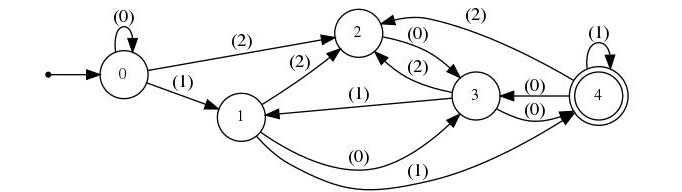
\includegraphics[width=\textwidth]{sturmian_word_paper/paper_images/theorem29C2.jpg}
    \caption{Automaton accepting lexicographically least sequence in shift orbit closure of $\Ctwo$}
\end{figure}
The proof for the lexicographically greatest is as follows, \newline 

Like we did for the lexicographically least, we need to create a predicate $P(n)$ for the lexicographically greatest sequence. 
\begin{equation*}
    \exists j\ C[j+n-1]=1\ \wedge\ \forall k\ ((\forall s \leq n\ C[j+s]=C[k+s])\ \vee \ (\exists i \leq n\ s.t.\ C[j+i] > C[k+i]\ \wedge
\end{equation*} 
$(\forall t < i\ C[j+t]=C[k+t])))$ \newline \\
The above predicate encodes that $b_{n}=1$ and that $b_{0}...b_{n}$ is equal to or lexicographically greater than t, where t is any length - (n + 1) factor of C = \Ctwo\ or \Cthree.\\  \newline
\begin{figure}[h]
    \centering
    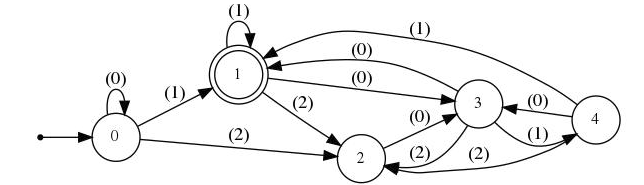
\includegraphics[width=\textwidth]{sturmian_word_paper/paper_images/theorem29greatest.png}
    \caption{Automaton accepting lexicographically greatest sequence in shift orbit closure of $\Ctwo$}
\end{figure} \newline
When we do this for C = \Ctwo, we get the above automaton, which can be seen to generate the sequence $1\Ctwo$. \\
\end{proof}


\subsection{Minimal forbidden words}

% Note: reference for definition: 
% [33] J. D. Currie, N. Rampersad, and K. Saari. Suffix conjugates for a class of morphic
% subshifts. In J. Karhumäki, A. Lepistö, and L. Zamboni, editors, WORDS 2013, Vol.
% 8079 of Lecture Notes in Computer Science, pp. 95–106. Springer-Verlag, 2013.

For some word $w$, the word $z$ is said to be \textit{forbidden} if it is not a factor of $w$.
A word $z$ is a \textit{minimal forbidden word} if it is a forbidden word of the form $a \cdot u \cdot b$, where $a$ and $b$ are symbols, such that $a \cdot u$ is a factor of $w$ and $u \cdot b$ is a factor of $w$.
That is, removing either the first or the last symbol of $z$ makes it a factor of $w$.

We can characterize the minimal forbidden words of $C_{\sqrt{2}}$ by creating an automaton which accepts pairs $(i,n)_{\sqrt{2}}$ such that $z = C_{\sqrt{2}}(i,n) \overline{C_{\sqrt{2}}[i + n]}$ is not a factor of $C_{\sqrt{2}}$, but $C(i + 1,n-1)\overline{C_{\sqrt{2}}[i+n]}$ is.
Then our minimal forbidden word is $z = a \cdot u \cdot b$, where $a = C_{\sqrt{2}}[i]$, $u = C_{\sqrt{2}}(i+1,n-1)$, and $b = \overline{C_{\sqrt{2}}[i + n]}$.
% Recall that $\overline{C_{\sqrt{2}}[n]}$ is the complement of $C_{\sqrt{2}}[n]$, so if $C_{\sqrt{2}}[n] = 0$, then $\overline{C_{\sqrt{2}}[n]} = 1$, and vice versa.
Clearly $a \cdot u = C_{\sqrt{2}}(i,n)$ is a factor of $C_{\sqrt{2}}$.
So all we need to check is that the whole word $z$, is not a factor of $C_{\sqrt{2}}$ and that $u \cdot b$ is a factor.

We then want an automaton accepting pairs $(i, n)$ such that $\text{MinimalForbidden}(i, n)$, defined below, holds.

\begin{equation*}
    \text{MinimalForbidden}(i, n) := \text{Forbidden}(i, n) \text{ and } \forall j < i, \neg \text{Forbidden}(j, n)
\end{equation*}

where $\text{Forbidden}(i,n)$ is

\begin{equation*}
\begin{split}
    \text{Forbidden}(i, n) :=~& n > 1 \text{ and }  \\
                     & (\forall j, ~\Ctwo(j,k) \neq \Ctwo(i,k) \text{ or }
                                  \Ctwo[j + n] \neq \overline{\Ctwo[i + n]}) ~ \text{and} ~ \\
                     & (\exists j, ~\Ctwo(j,k) = \Ctwo(i,k) ~ \text{and} ~
                                \Ctwo[j + n] \neq \Ctwo[i + n])
\end{split}
\end{equation*}

The second line of $\varphi$ ensures that the whole word, $z$, is not a factor of $\Ctwo$.
The third line ensures that $u \cdot b$, $z$ without its first symbol, is a factor of $\Ctwo$.

\begin{figure}
    \centering
    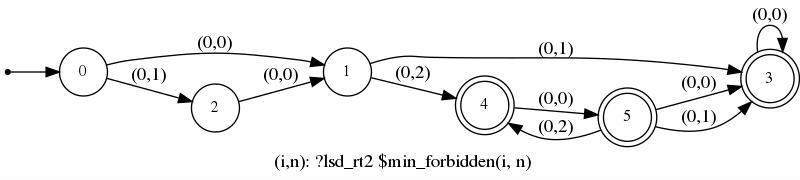
\includegraphics[width=\textwidth]{paper_images/minimal_forbidden_words.jpg}
    \caption{The location $i$ of the minimal forbidden factor with length $n$ in $C_{\sqrt{2}}$}
    \label{fig:min_forbidden_rt2}
\end{figure}

Walnut produces the automaton in Figure~\ref{fig:min_forbidden_rt2}, indicating the pairs of the positions $i$ and lengths $n$ for which $\Ctwo$ has minimal forbidden words.

% The analogous automaton for $\Cthree$ is shown in Figure~\ref{fig:min_forbidden_rt3}.

% \begin{figure}
%     \centering
%     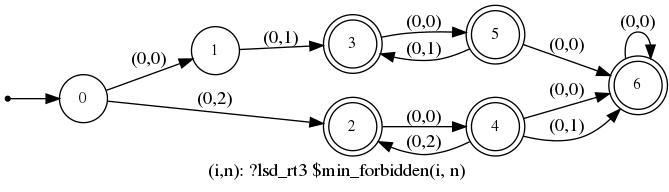
\includegraphics[width=\textwidth]{paper_images/minimal_forbidden_words_rt3.jpg}
%     \caption{The location $i$ of the minimal forbidden factor with length $n$ in $C_{\sqrt{3}}$}
%     \label{fig:min_forbidden_rt3}
% \end{figure}
